\documentclass{report}
% Balíky
\usepackage[czech]{babel}
\usepackage[IL2]{fontenc}
\usepackage[a4paper, total={6in, 8in}]{geometry}
\usepackage[utf8]{inputenc}
\usepackage{graphicx}
\usepackage{hyperref}

\hypersetup{
    colorlinks=true,
    linkcolor=black,
    filecolor=black,      
    urlcolor=blue,
    pdftitle={Sharelatex Example},
    bookmarks=true,
    }  
    
\title{Detekce potenciálů horních končetin v EEG záznamu}
\author{Jan Rubáš, Jan František Sedláček, Tomáš Vaněček}
\date{KIV/ZSWI LS 2019/20}
%
\begin{document}

\maketitle
\tableofcontents
%
\chapter{Specifikace požadavků}
Přizpůsobení jednoho (blíže nespecifikovaného) scénáře z OpenVibe již existujícím naměřeným datům tak, aby byl schopen na základě těchto dat klasifikovat pohyby horních končetin (levou a pravou rukou).
Obecný postup pro testování scénáře.
Nalezení základních požadavků na funkční scénář.

\section{Popis a priorita}
Úprava scénáře z prostředí OpenVibe tak, aby byl schopen pracovat s naměřenými daty, klasifikovat druh pohybu horních končetin a zjistit do jaké míry je schopen tento pohyb klasifikovat.

\subsection{Události a odpovědi}
Klasifikátor bude schopen z naměřených dat identifikovat pohyb jedné z horních končetin.

V případě, že nebude umožněn přístup do laboratoře UN323 po 13.4.2020, tak se použijí již naměřená data, podle kterých se jeden z již existujících scénářů přizpůsobí.

\subsection{Funkční požadavky}
Kvalitní vstupní offline data:
Spolupracující a čilý subjekt.
Správně připravené nástroje (ECI čepice, BrainApm DC, pracovní stanice... )
Správně připravené prostředí pro testování.
\\
\\
\\
\\
\\
\\
Podrobnější specifikace celého projektu je popsaná v dokumentu
\href{https://docs.google.com/document/d/1LbMN5tFxxpSZ1Gf7irw77nM88PaOCfTKEih6rNO8mn0/edit?usp=sharing}{Specifikace projektu}.


\chapter{Analýza problému a návrh programu}
%
\section{Konvertování}
%
Scénář bude pomcí pluginu \textit{BrainVision Format file reader} načítat původní  \textit{.vhdr, .eeg, .vmrk} offline soubory a bude je konvenrtovat na formát \textit{.ov}, který podporuje rozhraní OpenVibe.
%
\section{Trénování}
Scénář bude určený pro generování trénovací množiny dat.

Bude filtrovat vstupní kanály a zuží je pouze na čtyři - \textbf{C3, C4, P3, P4}. Tyto kanály obsahují veškeré informace o pohybu horních končetin.

Vstup pro tento scénář budou \textit{.ov} soubory a výstupem bude jeden prvek trénovací množiny \textit{.cfg}.
%
\section{Testování klasifikace}
Scénář bude určený pro klasifikaci scénáře na základě trénovací množiny.

Jeho vstupem bude \textit{.ov} soubor, který se bude klasifikovat a trénovaná množina souborů \textit{.ov} na jejíž základě se bude vyhodnocovat, jak moc je tento klasifikátor úspěšný.
\\
\\
\\
\\
\\
\\
Podrobná analýza našeho projektu a jeho následná implementace je popsána v dokumentu
\href{https://docs.google.com/document/d/1DZhPO0-b6VwDLwlwbTCjLrkphk3x23aponyvLbC3uOU/edit?usp=sharing}{Strukturovaná analýza projektu}.


\chapter{Uživatelská dokumentace}
\section{Spuštění}
Před spuštění projektu je potřeba otevřít zdrojové kódy scénářů pro convertování, trénování a testování dat v rozhraní OpenVibe pomocí \textbf{File - Open - "vybraný soubor"}.

 
\section{Nahrání dat do scénářů}
Po otevření scénářů je potřeba nahrát data, se kterými budeme pracovat.
\subsection{convert.xml}
 Používáte-li data s příponou \textit{.vhdr, .eeg, .vmrk} (tyto soubory jsou vzájemně propojeny, proto je potřeba mít v jedné složce všechny tyto soubory), je třeba tato data konvertovat do openvibe formátu \textit{.ov}. Cestu k \textit{.vhdr} souboru načtete po kliknutí na plugin \textit{Brainamp file reader} a cestu nastavíte okénku \textit{Filename} a stisknete tlačítko \textit{Apply} (viz obrázky: \ref{fig:converter} a \ref{fig:filereader})
 
 Cestu, kam chceme uložit výsledný soubor v \textit{.ov} formátu nastavíme po kliknutí na plugin \textit{Generic stream writer}. Zobrazí se dialogové okno s nastavením cesty a názvu souboru, kam jej chceme uložit v poli \textit{Filename} (viz obrázek \ref{fig:filewriter}). 

 Dále nastavíme manuálně pomocí pluginu časovače \textit{Timeout} časový úsek od počátku záznamu původního \textit{.vhdr} souboru, který chceme konvertovat (musíme si také uvědomit časovou náročnost měření, která je zaznamenána v souboru \textit{.vhdr} a podle toho nastavit příslušný čas, viz obrázek \ref{fig:timeout}).
 
 Celý tento scénář pustíme pomocí tlačítka symbolizující \textbf{start/play šipku} na obrázku a rychlost přehrávání, případné zastavení ovládáme pomocí vedlejších tlačítek \ref{fig:btns}. Zobrazí se nám naměřený EEg signál, který je uložený v \textit{.vhdr} souboru.
 %
\begin{figure}[!ht]
\centering
  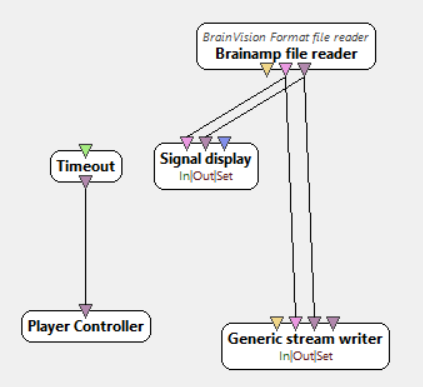
\includegraphics[width=0.3\textwidth]{pictures/coverter.png}
  \caption{Scénář converter}
  \label{fig:converter}
 \end{figure}
 %
\begin{figure}[!ht]
\centering
  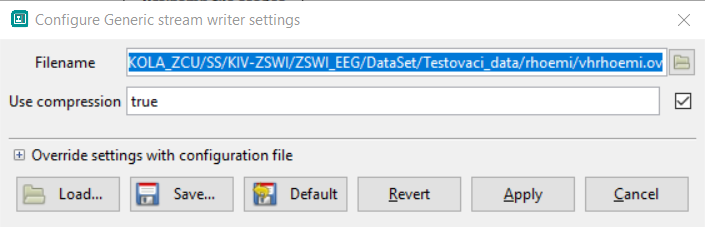
\includegraphics[width=0.5\textwidth]{pictures/setFileReader.png}
  \caption{Nastavení Brainamp file reader}
  \label{fig:filereader}
 \end{figure}
 %
 \begin{figure}[!ht]
\centering
  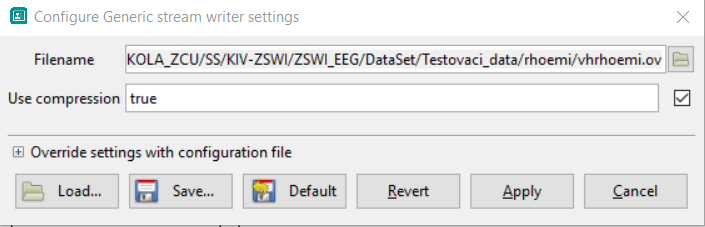
\includegraphics[width=0.5\textwidth]{pictures/configurewriter.png}
  \caption{Nastavení Generic stream writer}
  \label{fig:filewriter}
 \end{figure}
 %
 \begin{figure}[!ht]
\centering
  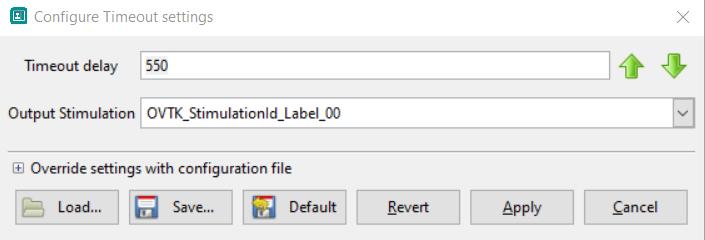
\includegraphics[width=0.5\textwidth]{pictures/timeout.png}
  \caption{Nastavení zpoždění}
  \label{fig:timeout}
 \end{figure}
 %
  \begin{figure}[!ht]
\centering
  
\includegraphics[width=0.3\textwidth]{pictures/playstart.png}
  \caption{Ovladač přehrávání a konvertování}
  \label{fig:btns}
 \end{figure}

\subsection{trainer.xml}
Scénář určený pro trénování. V pluginu \textit{Generic stream reader} nastavíme vstupní soubor \textit{.ov} formátu obdobně jako jsme nastavovali vstupní soubor v \textbf{convert.xml}, který chceme natrénovat.

V pluginu \textit{Classifier trainer} a jeho textovém poli \textit{Filename to save configuration to} nastavíme příslušný soubor a cestu, kam trénovací soubor uložit v \textit{.cfg} formátu (obrázek \ref{fig:trainer}).

  \begin{figure}[!ht]
\centering
  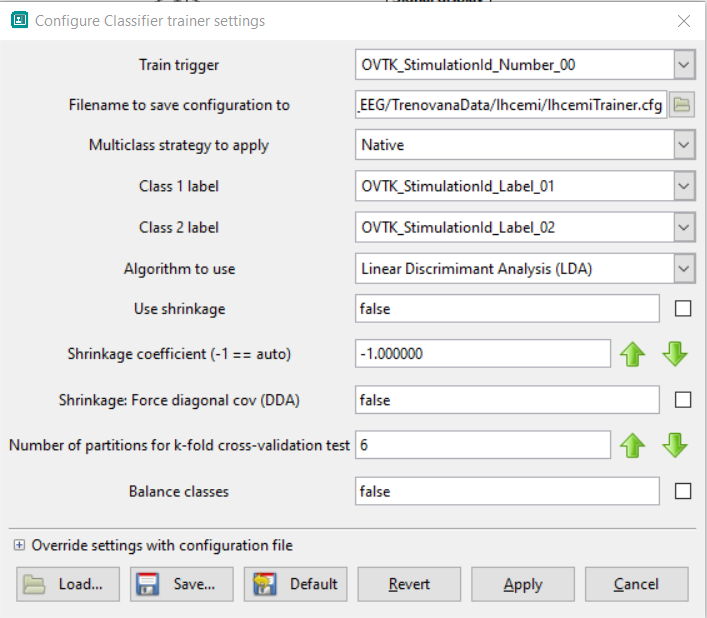
\includegraphics[width=0.5\textwidth]{pictures/trainer.png}
  \caption{Classifier trainer}
  \label{fig:trainer}
 \end{figure}

Nakonec spustíme scénář stejným způsobem jako při konverzi dat.
\subsection{testing.xml}
Scénář sloužící ke klasifikaci dat.

Nejdříve musíme nastavit cestu ke klasifikovanému souboru. Stejně jako u \textbf{trainer.xml} nastavíme \textit{Generic stream reader}.
V pluginu \textit{Classifier processor} nastavíme v poli \textit{Filename to load coniguration from} cestu, kde se nachází trénovací soubor v \textit{.cfg} formátu (obrázek \ref{proc}.

Nyní můžeme tento scénář spustit a zobrazí se nám výsledky klasifikace a zkoumaný signál.

 %
  \begin{figure}[!ht]
\centering
  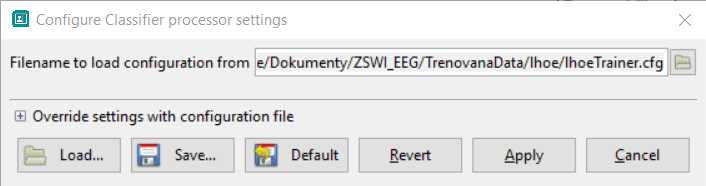
\includegraphics[width=0.5\textwidth]{pictures/processorclass.png}
  \caption{Classifier processor}
  \label{fig:btns}
 \end{figure}


\chapter{Závěr}
Ačkoli nám uzavření fakulty znemožnilo realizovat původní zadání s využitím online měřených dat, byli jsme nuceni požádat zadavatele o přizpůsobení původního zadání těmto změnám. Nakonec se nám podařilo zrealizovat scénáře pro klasifikaci potenciálů horních končetin z již existujicích offline dat.
\end{document}

